\documentclass{article}

\title{Super iper-mega bigliettino per l'esame scritto di misure elettroniche}
\author{Stefano Rossini}

\usepackage{bookmark}

\usepackage[italian]{babel}
\usepackage{geometry}
%\geometry{a4paper, margin={2.54cm,1.9cm}}
\geometry{a4paper, margin={0.1cm,0.1cm}}
\usepackage{hyperref}
\usepackage{tcolorbox} %for COLORED BOXES 

\usepackage{amsmath}
\usepackage{graphicx}
\graphicspath{{./immagini/}}

\usepackage{url}

\usepackage{physics}

\usepackage{amsfonts} 

\usepackage{gensymb}

\usepackage{textcomp}

\usepackage{tikz}

\usepackage{pgfplots}

\usepackage{multicol}

\begin{document}
\begin{multicols*}{3}
    \textbf{Multipli e sottomultipli} \newline
    \begin{tabular}{c c c}
        Nome & Simbolo & Moltiplicazione \\
        exa & E & $10^{18}$ \\
        peta & P & $10^{15}$ \\
        tera & T & $10^{12}$ \\
        giga & G & $10^{9}$ \\
        mega & M & $10^{6}$ \\
        kilo & k & $10^{3}$ \\
        etto & h & $10^{2}$ \\
        deca & da & $10^{1}$ \\
        deci & d & $10^{-1}$ \\
        centi & c & $10^{-2}$ \\
        milli & m & $10^{-3}$ \\
        micro & $\mu$ & $10^{-6}$ \\
        nano & n & $10^{-9}$ \\
        pico & p & $10^{-12}$ \\
        femto & f & $10^{-15}$ \\
        atto & a & $10^{-18}$
    \end{tabular}
    \newline 
    N = valori di ripetizioni della misura  \newline 
    \textbf{Valore medio:}  
    $\overline{x} = \frac{1}{N} \sum_{k=1}^{N} x_k$ \newline
    \textbf{Deviazione dal valor medio \\ (scostamento):}
    $\delta_k = x_k - \overline{x}$ \newline
    \textbf{Varianza speimentale:} \\
    $s^{2}(x_k) = \frac{1}{N-1} \sum_{k =1}^{N} \delta_k ^{2}$ \newline 
    \textbf{Scarto tipo sperimentale:}\\
    $s(x_k) = \sqrt{s^{2} (x_k)}$ \newline 
    \textbf{Scarto (deviazioni) tipo $\sigma$:}\\
    $\pm 1 \sigma = 68.27 \%$ , $\pm 2 \sigma = 95.45 \%$ , \\ 
    $\pm 3 \sigma = 99.73 \%$ \newline
    \textbf{Scarto tipo del valor medio \\ sperimentale:} \\ 
    $s(\overline{x}) = \frac{s(x_k)}{\sqrt{N}} = \sqrt{\frac{1}{N (N-1)} \sum_{k=1}^{N} (x_k - \overline{x})^{2}}$ \newline 
    \hrule
    \textbf{VALUTAZIONE DI TIPO A} \newline
    \textbf{Incertezza (uncertainty):}\\
    $u_A(\overline{x}) ^{2} = s^{2} (\overline{x})$ in termini di varianza, \\
    $u_A(\overline{x}) = s (\overline{x})$ in termini di scarto tipo \newline
    \textbf{VALUTAZIONE DI TIPO B} \newline
    $[-a, +a]$ intervalllo centrato sul valore medio $\overline{x}$ \\
    Se PDF uniforme $\to$ $u_B (\overline{x}) = \frac{a}{\sqrt{3}}$ \\ 
    Se PDF triangolare $\to$ $u_B (\overline{x}) = \frac{a}{\sqrt{6}}$ \\ 
    Se PDF gaussiana $\to$ $u_B (\overline{x}) = \frac{a}{3}$ \newline 
    \textbf{Incertezza combinata standard:}\\
    $u_C (\overline{x}) = \sqrt{u_A ^{2} (\overline{x}) + u_B ^{2} (\overline{x})}$ \newline 
    \textbf{Incertezza estesa:} \\
    $U(\overline{x}) = k \cdot u_C (\overline{x})$ \\
    in cui k = fattore di copertura (numero intero) \newline
    p = probabilità di copertuta \newline 
    Se k = 1 $\leftrightarrow$ p $\approx$ 68 \% \\
    Se k = 2 $\leftrightarrow$ p $\approx$ 95 \% \\
    Se k = 3 $\leftrightarrow$ p $\approx$ 99 \% \newline
    \textbf{GRANDEZZA CALCOLATA IN MODO INDIRETTO y}\newline 
    y è una grandezza calcolata indirettamente che è funzione di altre grandezze: \\
    y = f($x_1$, $x_2$, ... ,$x_m$ ) \newline
    \textbf{Incertezza tipo composta:} \\
    $u_C (y) = \sqrt{\sum_{i = 1}^{m} \left( \frac{\partial f(x_1, x_2, ... ,x_m )}{\partial x_i}\right)^{2} \cdot u_C ^{2} (x_i)}$ \newline
    \hrule 
    \textbf{STRUMENTI DIGITALI} \newline 
    incertezza strumentale (accuracy), in forma binomiale: \\
    a = $\Delta_g = \pm (c \%  \cdot \overline{x} + b \cdot $\text{ digit}$)$ \newline 
    a andrà sostituita nella formula di $u_B (\overline{x})$ \newline 
    Se non viene indicata una PDF dello strumento, \\
    utilizzare PDF uniforme \newline 
    \textbf{Incertezza assoluta:}\\
    $\Delta x = \pm U$ \newline
    \textbf{Incertezza relativa:}\\
    $\frac{\Delta x}{x} = \pm \frac{U}{x}$ \newline 
    \textbf{Incertezza percentuale:}\\ 
    $\Delta x \% = \pm 100 \cdot (\frac{U}{x})$ \newline 
    \textbf{Incertezza relativa in ppm (parti per milione):}\\ 
    $\frac{\Delta x}{x}$ (ppm) = $\pm 10^{6} \cdot (\frac{U}{x})$ \newline 
    \textbf{CIFRE SIGNIFICATIVE \\ (APPROSSIMAZIONI)}: \\
    Si parte da U intervallo. 
    Si può scegliere 1 o 2 cifre contigue (attaccate, vicine) diverse da zero (partendo da sinistra). 
    U si arrotonda SEMPRE per eccesso (la cifra da approssimare aumenta di 1), 
    x al valore più vicino (cioè se la cifra a destra della cifra da approssimare è maggiore di 5, la cifra aumenta di 1; se è il contrario rimane come è) \newline 
    Dato il k dall'esercizio, moltipilcare l'incertezza assoluta calcolata e, solo alla fine, approssimare alle cifre significative dato dall'esercizio. \newline
    \textbf{COMPATIBILITA' TRA LE \\ MISURE} \\
    \textbf{Metodo grafico:} \\
    si può disegnare e graficare la misura disegnando una retta e ponendo il valore centrale delle misure ed i loro intervalli: 
    se gli intervalli si sovrappongono, anche solo gli estremi, le misure sono compatibili \newline 
    \textbf{Metodo analitico:} \\
    Date due misure, con i loro valori centrali $x_1$, $x_2$ con le loro incertezze $u(x_1)$, $u(x_2)$, 
    due misure sono compatibili se: \\
    $\abs{x_1 - x_2} \leq \alpha \sqrt{u(x_1) ^{2} + u(x_2) ^{2} }$ \\
    dove $\alpha$ è il fattore di ricopertura($\alpha$ deve essere un numero intero). \\
    Per essere una buona misura, si accettano valori di $\alpha$ da 1 a 3 compresi. \newline 
    Inoltre, può essere richiesta la media pesata tra i valori. \\
    Date L misure compatibili, la media pesata è: \\
    $\overline{x_{MP}} = \frac{\sum_{l = 1}^{L} \frac{x_l}{u^{2}(x_l)}}{\sum_{l = 1}^{L} \frac{1}{u^{2}(x_l)}}$ \newline 
    L'incertezza della media pesata vale: \\
    $u^{2} (\overline{x_{MP}}) = \frac{1}{\sum_{l = 1}^{L} \frac{1}{u^{2}(x_l)}}$
    \hrule
    \textbf{MISURA VOLTAMPEROMETRICA} \newline
    \textbf{Misura di resistenza con voltmetro a valle:} \\
    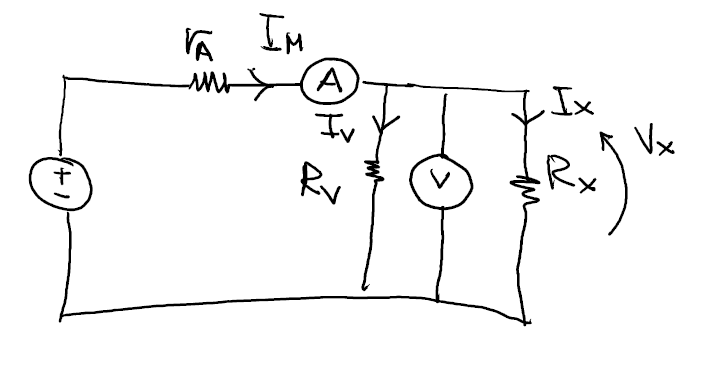
\includegraphics[scale = 0.5]{Valle.PNG}
    $R_m = \frac{V_m}{I_m} = \frac{V_m}{I + I_v} = \frac{V_m}{I + \frac{V_m}{R_v}} < \frac{V_m}{I} = R_x $ \\
    oppure, in termini solo di resistenze: \\ 
    $R_x = \frac{R_m}{1 - \frac{R_m}{R_v}}$ \\
    dove $R_v$ è la resistenza del voltmetro, $r_A$ è la resistenza dell'amperometro, $R_x$ è la resistenza nominale del bipolo da misurare, $R_m$ è la resistenza misurata \newline
    \textbf{Misura di resistenza con voltmetro a monte:} \\
    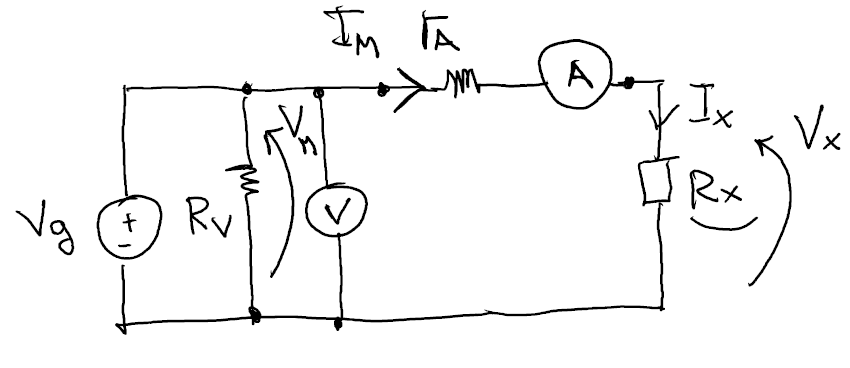
\includegraphics[scale = 0.44]{Monte.PNG}\\
    $R_m = \frac{V_m}{I_m} = \frac{V + r_a \cdot I_m}{I_m} > \frac{V}{I_m} = R_x $ \\
    oppure, in termini solo di resistenze: \\ 
    $R_x = R_m - r_A$ \\
    dove $R_v$ è la resistenza del voltmetro, $r_A$ è la resistenza dell'amperometro, $R_x$ è la resistenza nominale del bipolo da misurare, $R_m$ è la resistenza misurata \newline
    \hrule
    \textbf{ELETTROTRCNICA} \newline 
    \textbf{Legge di Ohm:} \\ 
    $V = R \cdot I$ \newline 
    \textbf{Calcolo della potenza:} \\
    $P = V \cdot I$ \newline
    \textbf{Circuito equivalente di Norton:} \\
    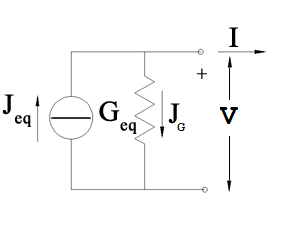
\includegraphics[scale = 0.3]{Norton.png} \newline 
    \textbf{Circuito equivalente di Thevenin:} \\ 
    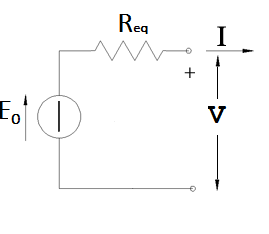
\includegraphics[scale = 0.3]{Thevenin.png} \newline 
    \hrule 
    \textbf{DERIVATE}\newline 
    \textbf{Derivate semplici:} \\
    $\frac{d}{dx} x^{\alpha} = \alpha x ^{\alpha -1}$\\
    $\frac{d}{dx} \alpha ^{x} = \ln(\alpha) \alpha^{x} $ \\
    $\frac{d}{dx} \log_{\alpha} (x) = \frac{1}{x \ln(\alpha)} $ \\
    $\frac{d}{dx} \ln(x) = \frac{\abs{x}}{x} $ \\
    $\frac{d}{dx} e^{x} = e^{x} $ \\
    $\frac{d}{dx} \sin(x) = \cos(x)$ \\
    $\frac{d}{dx} \cos(x) = - \sin(x)$ \\
    $\frac{d}{dx} \tan(x) = \frac{1}{\cos^{2} (x)} = 1 + \tan^{2} (x)$ \newline
    \textbf{Regole di derivazione:} \\ 
    $(k \cdot f(x))^{'} = k \cdot f(x)^{'}$ \\ 
   $(f(x) \pm g(x))^{'} = f^{'} (x) \pm g^{'} (x)$ \\ 
   $(f(x) \cdot g(x) )^{'} = f^{'} (x) \cdot g(x) + f(x) \cdot g^{'} (x)$ \\ 
    $(\frac{f(x)}{g(x)})^{'} = \frac{f^{'} \cdot g(x) - f(x) \cdot g^{'} (x)}{g^{2} (x)}$ \\ 
    $(\frac{1}{f(x)})^{-1} = - \frac{f^{'}}{f^{2} (x)}$ \\ 
    $[f(g(x))]^{'} = f^{'} (g(x)) \cdot g^{'} (x)$ \newline
    \textbf{Derivate di funzioni composte:} \\
    $D[f(x)]^{\alpha} = \alpha [f(x)]^{\alpha -1} \cdot f^{'} (x)$\\
    $D \log(f(x)) = \frac{f^{'} (x)}{f(x)}$ \\
    $D \text{ } \alpha^{f(x)} = f^{'} (x) \cdot \alpha ^{f(x)} \cdot \ln(\alpha)$ \\
    $D \text{ } e^{f(x)} = f^{'} (x) \cdot e^{f(x)} $ \\
    $D  \text{ } \sin(f(x)) = f^{'} (x) \cdot \cos(f(x)) $ \\
    $D  \text{ } \cos(f(x)) = f^{'} (x) \cdot - \sin(f(x)) $ \\
    $D  \text{ } \tan(f(x)) = \frac{f^{'} (x)}{\cos^{2} (f(x))}$ \newline
    \hrule 
    \textbf{REGOLA PER FARE LE DERIVATE PARZIALI:} \\
    considera tutte le altre variabili come costanti rispetto alla variabile in cui fare la derivata \newline 
    \hrule 
    \textbf{FORMULARIO SCRITTO MISURE ELETTRONICHE } \newline
\end{multicols*}
\end{document}